
\documentclass[11pt]{article}


\usepackage{fullpage}
\usepackage{amsmath}
\usepackage{amssymb}
\usepackage{algorithm}
\usepackage{algpseudocode}

\usepackage{verbatim}

\usepackage[scr=boondoxo]{mathalfa}

\usepackage{graphicx}
\usepackage{xcolor}

\usepackage{pdfpages}

\usepackage[round]{natbib}

\newcommand{\N}{\mathcal{N}}
\newcommand{\A}{\mathcal{A}}
\newcommand{\Z}{\mathcal{Z}}
\newcommand{\tff}{t^{\mathrm{ff}}_{ij}}


\usepackage[colorlinks=true]{hyperref}
\hypersetup{%
	urlcolor=blue,% hyperlink text will be green
	linkcolor=black,
	citecolor=black,
	filecolor=black
}


\DeclareMathOperator*{\argmin}{\arg\min}



\begin{document}
	\allowdisplaybreaks[1]
	
	
	\title{CEGE 3201: Static traffic assignment in Python}
	
	\author{Michael W. Levin}
	
	
	
	\maketitle
	
	
	\section{Introduction}
	
	The purpose of this lab is to implement a basic traffic assignment algorithm to better understand how computers are used to solve traffic assignment. This lab is written in Python 3, so you will first need to set up some version of Python 3 on your computer to run it. (Note that Python versions 1 and 2 are not compatible with this lab due to the object-oriented code.) This lab will list specific exercises of code implementation that are designed to be completed sequentially as they build on the code written previously. 
	
	
	Download a copy of this Git repository: \href{https://github.com/mwlevin/STA_python_3201.git}{https://github.com/mwlevin/STA\_python\_3201.git}. 
	The repository contains 4 folders.
	\begin{itemize}
		\item The ``documentation'' folder contains this explanation.
		\item The ``src'' folder contains the source files you will use and modify.
		\item The ``autograde'' folder contains code to automatically check the correctness of your work.
		\item The ``data'' folder contains some test data that will be used within this lab. If you are curious, you can find data for different cities in the same format at
		
		\noindent \href{https://github.com/bstabler/TransportationNetworks}{https://github.com/bstabler/TransportationNetworks}
		
		\noindent
		After you complete this lab, you will be able to solve traffic assignment on other networks (although your algorithm will be very basic, so it may take a long time).
	\end{itemize}
	
	The \texttt{main()} function (which is executed when you run the program) is found in main.py. Each of the exercises in this tutorial are contained within a separate file, e.g. Exercise1.py, Exercise2.py, etc. Each of these files has their own \texttt{test()} function that can be executed.
	In main.py, you will find calls to these functions \href{https://www.w3schools.com/python/python_comments.asp}{commented out}, i.e. \texttt{\#Exercise1.test()}. Uncomment them to run each exercise. 
	
	\begin{center}
		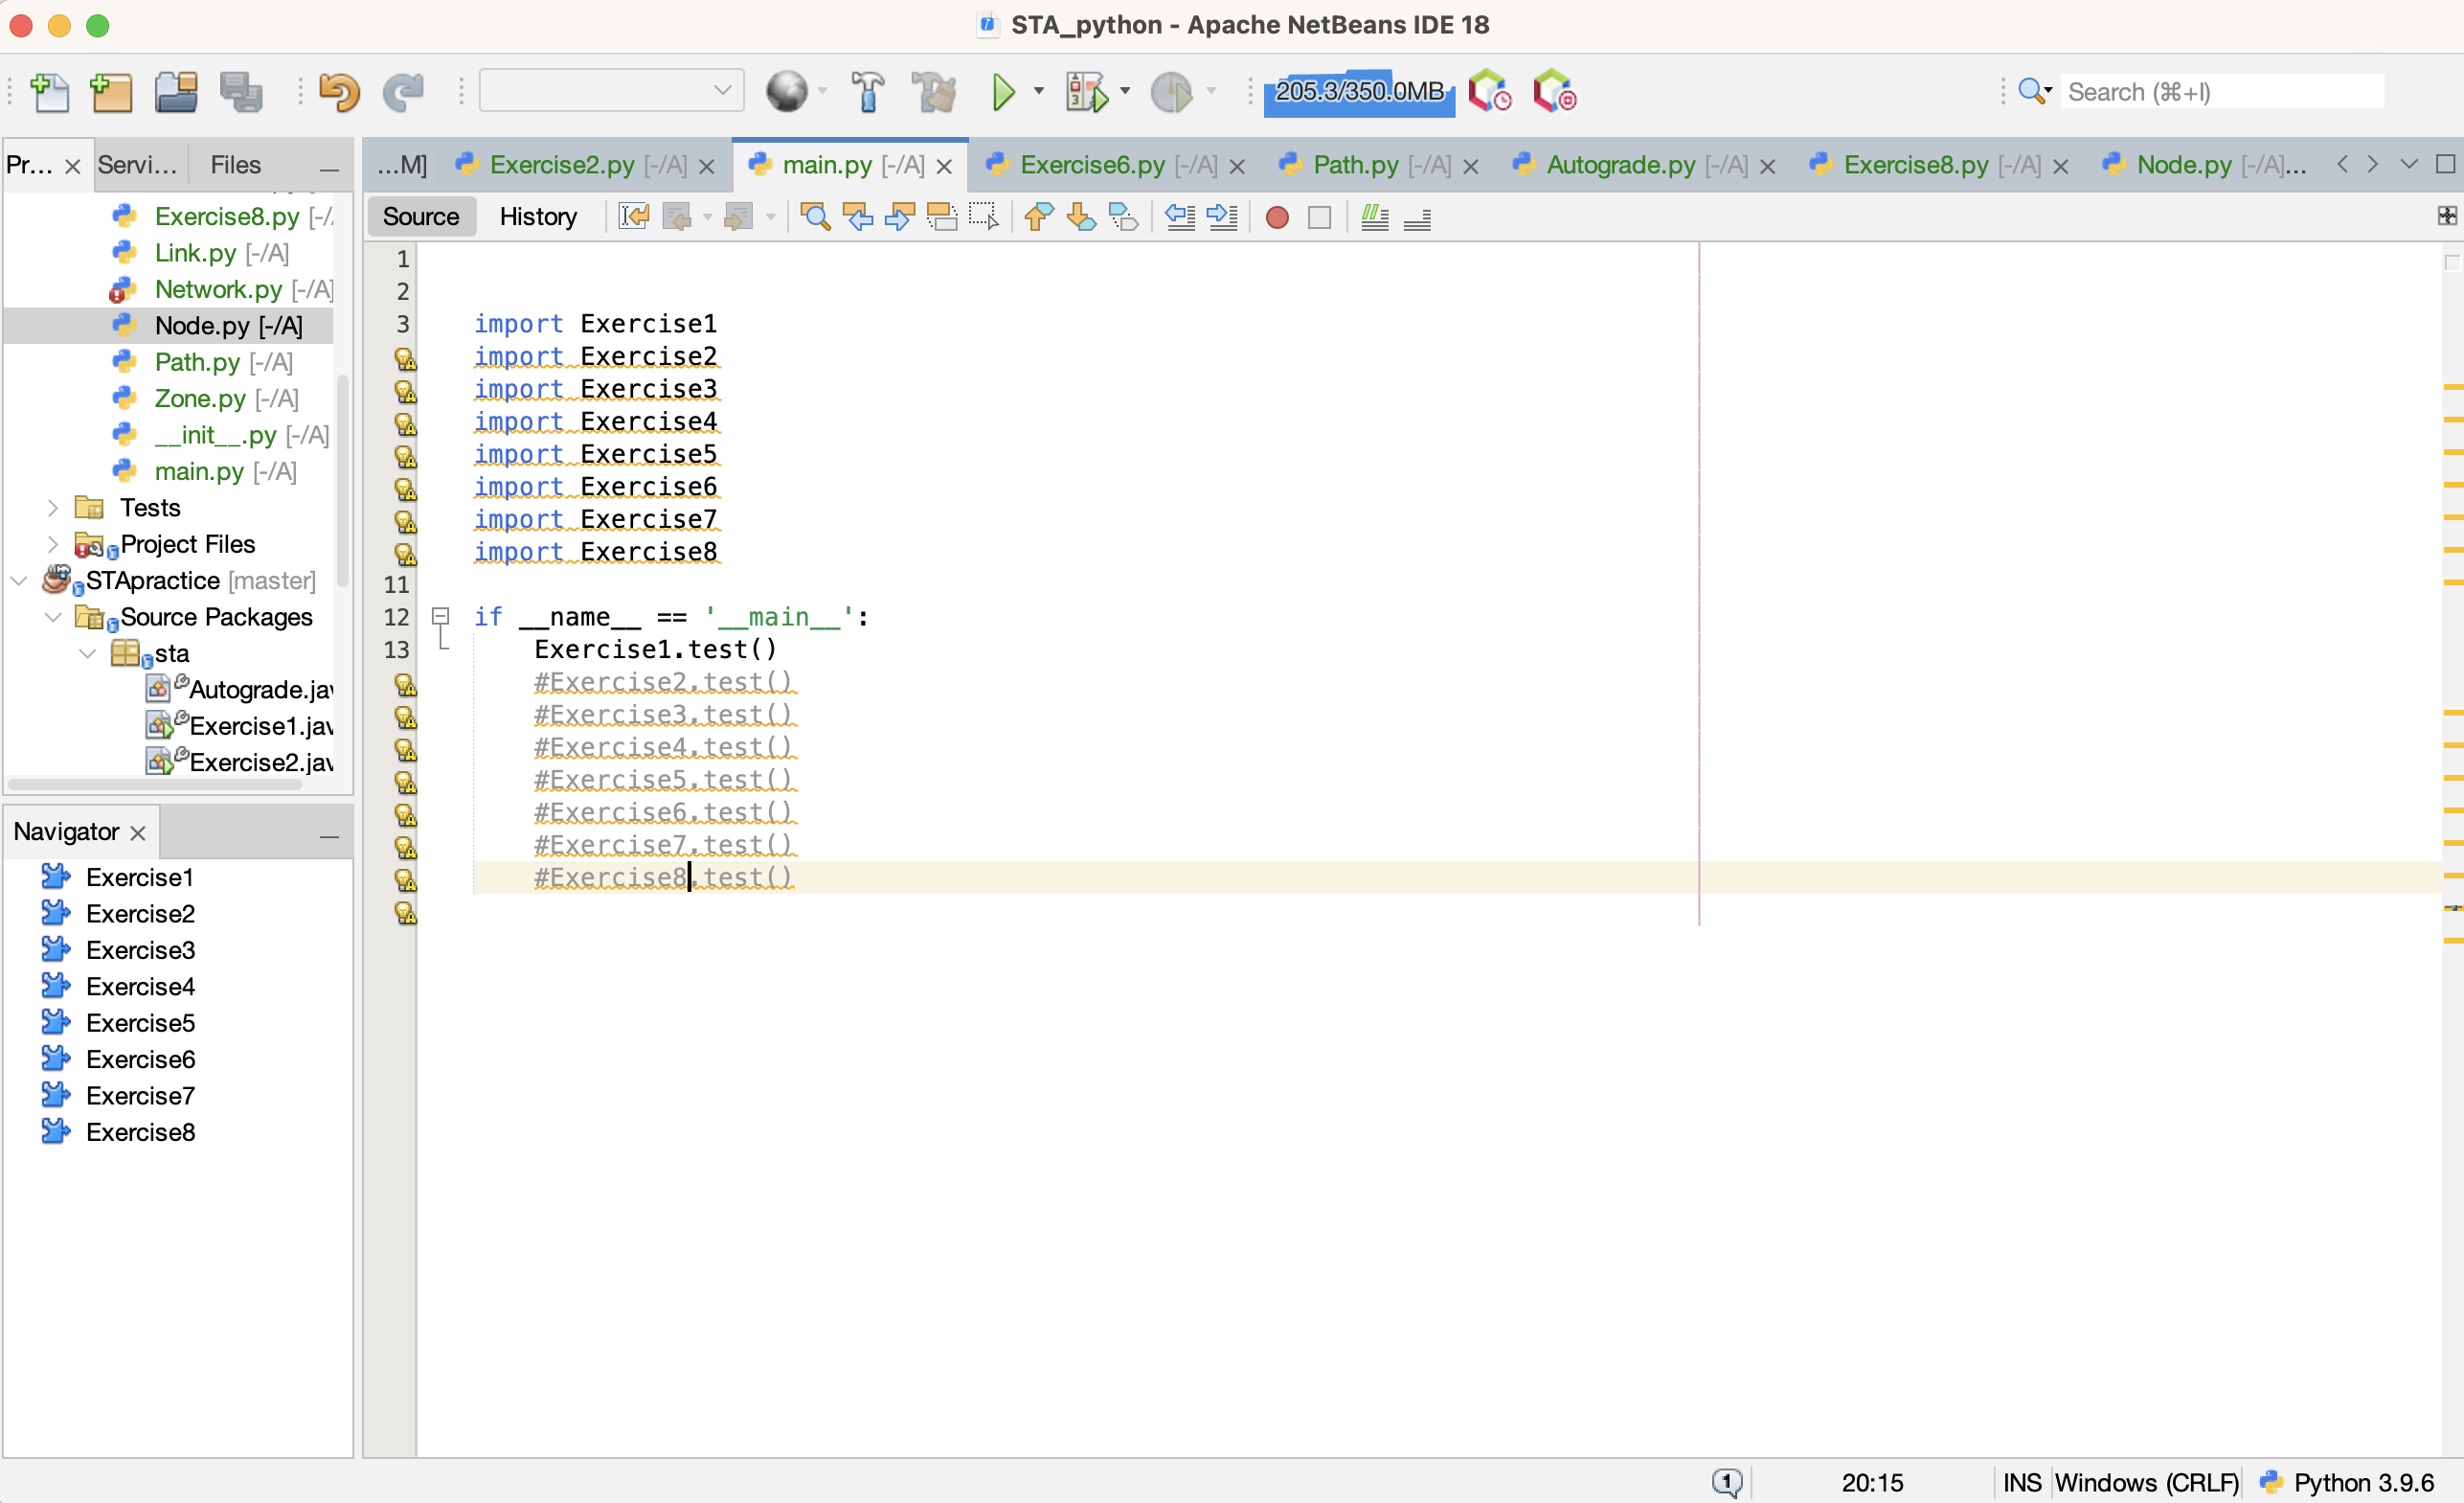
\includegraphics[width=\textwidth]{netbeans1.png}
	\end{center}
	
	Each exercise contains some test code. At the end of the \texttt{test()} function, it calls the \texttt{autograde()} function which will automatically test the output of your code against the correct answers. Go ahead and run the code; it should run successfully, but the autograde will indicate that your code is incorrect:
	
	\begin{center}
		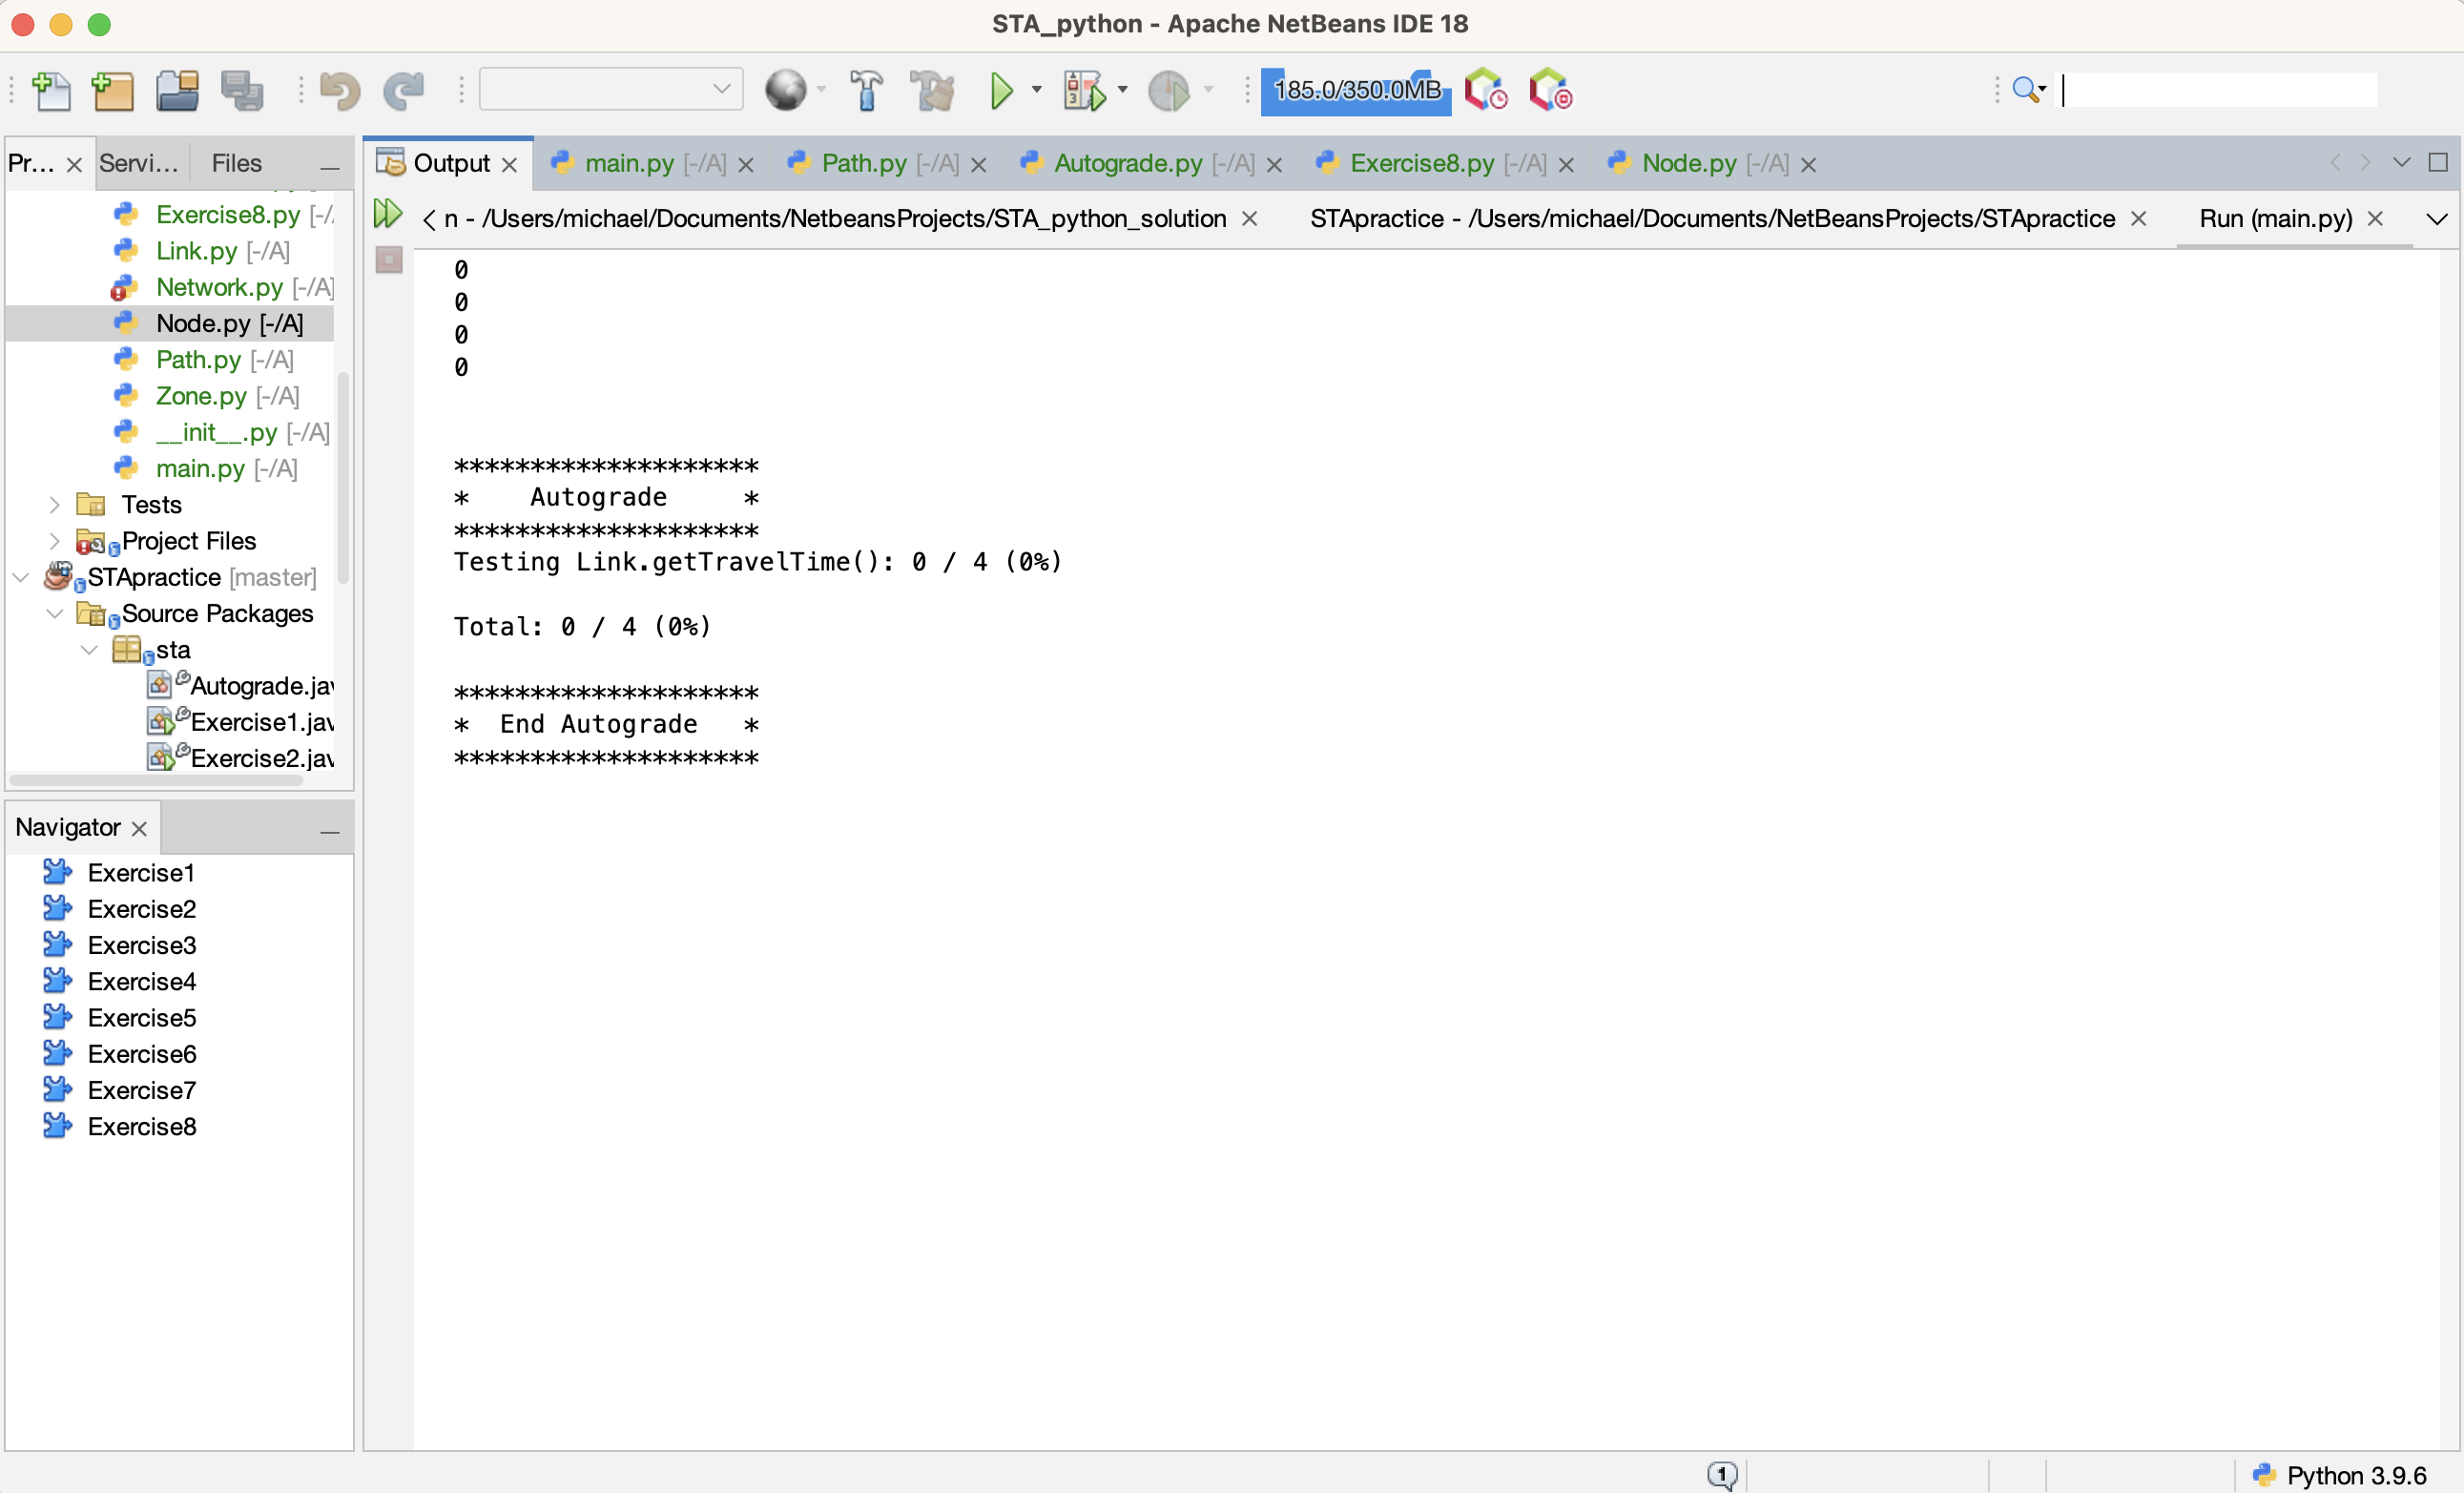
\includegraphics[width=\textwidth]{netbeans1a.png}
	\end{center}
	

\section{Calculating travel times}

We will use $(i,j)$ to refer to a link from node $i$ to node $j$, with $\A$ the set of all links. 

\paragraph*{Exercise 1(a)} Implement the calculation of the link travel time $t_{ij}(x_{ij})$ using the BPR function 
\begin{equation}
	t_{ij}(x_{ij}) = \tff \left(1+\alpha_{ij} \left(\frac{x_{ij}}{C_{ij}}\right)^{\beta_{ij}}\right) \label{bpr}
\end{equation}
 where $\tff$ is the free flow travel time, $C_{ij}$ is the link capacity, and $\alpha_{ij}$ and $\beta_{ij}$ are calibration constants.
You will see some variables \texttt{x}, \texttt{t\_ff}, \texttt{C}, \texttt{alpha}, and \texttt{beta} defined in the function \texttt{\_\_init\_\_()}. These variables are available for use anywhere within the \texttt{Link} class by using the \href{https://www.w3schools.com/python/gloss_python_self.asp}{``\texttt{self}'' reference}, and they contain the values you need. (These values have either been specified or read from one of the data files.)

Within the \texttt{Link} class in Link.py, find the function labeled \texttt{getTravelTime()}. It defines a variable \texttt{t\_{ij}} and sets the value to 0.0 --- a floating-point number. You need to calculate the correct value of $t_{ij}(x_{ij})$ and assign it to variable \texttt{t\_ij}. 


It may help to look at  \href{https://www.w3schools.com/python/python_syntax.asp}{Python syntax},  \href{https://www.w3schools.com/python/python_variables.asp}{variables} and \href{https://www.w3schools.com/python/python_datatypes.asp}{data types}. For math calculations, it may help to look at tutorials on \href{https://www.w3schools.com/python/python_operators.asp}{operators} and the \href{https://www.w3schools.com/python/python_math.asp}{math functions}. 

\begin{center}
	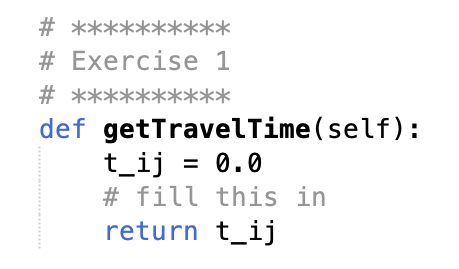
\includegraphics[width=0.3\textwidth]{netbeans3.png}
\end{center}

\noindent Open main.py and ensure that it will run \texttt{Exercise1.test()}.
Open autograde/Exercise1.py. The \texttt{main()} method constructs two instances of the \texttt{Link} class with different parameters. The first link has $t^{\mathrm{ff}}_{1}=10$, $C_{1}=2580$, $\alpha_{1}=0.15$, and $\beta_{1}=4$. The second link $t^{\mathrm{ff}}_{2}=12$, $C_{2}=1900$, $\alpha_{2}=0.35$, and $\beta_{2}=2$. The \texttt{main()} function then prints the calculation of $t_{ij}$ with $x_{1}=1230.2$, $x_2=570$, $x_1=0$, and $x_2=2512$. You should compare the values calculated by your code with values that you have computed by hand. 
Afterwards, \texttt{test()} calls the \texttt{autograde()} function, which runs an automated test of your answers. 


	
	
\paragraph*{Exercise 1(b)}  Open Network.py and implement the \texttt{getTSTT()} function to  return the total system travel time. The TSTT is defined as
\begin{align}
	TSTT = \sum_{(i,j)\in\A} x_{ij} t_{ij}(x_{ij})
\end{align}
The value for $x_{ij}$ is available from a variable in the Link class, and you wrote the method for $t_{ij}(x_{ij})$ in Exercise 1(a).
%
It may be helpful to look at tutorials on \href{https://www.w3schools.com/python/python_conditions.asp}{\texttt{if} statements}
 and \href{https://www.w3schools.com/python/python_for_loops.asp}{for loops} here.  Also, we are working with object-oriented programming, so it may be helpful to read the tutorial on \href{https://www.w3schools.com/python/python_classes.asp}{classes} to understand the interactions between the code. We will not ask you to implement any specific object-oriented code, but you will be working with \texttt{Node}, \texttt{Link}, and \texttt{Path} objects.


\vspace\baselineskip

\noindent
After completing Exercises 1(a)--1(b), your code should pass the \texttt{autograde()} method of Exercise1.py. 



\section{Dijkstra's shortest path algorithm}


We need to implement a shortest path algorithm, which will be used as a step in solving traffic assignment. We will implement the well-known Dijkstra's algorithm, which finds the one-to-all shortest path. We need to define two variables for this. Let $V(n)\in\mathbb{R}_+$ be the cost label of node $n$, and let $P(n)\in\N$ be the predecessor node. First, read through a pseudocode of this algorithm, which we also saw in class:


\vspace{\baselineskip}


\begin{algorithmic}[1]
	\Procedure{Dijkstra's}{$r$} 
	\For{$n\in \N$} \Comment{Initialization} \label{line1}
	\State $V(n) \leftarrow \infty$
	\State $P(n) \leftarrow \emptyset$
	\EndFor
	\State $c_r \leftarrow 0$ \label{line6}
	\State  $Q\leftarrow \{r\}$ \label{line7}
	
	\vspace{0.5\baselineskip}
	
	\While{$Q\neq\emptyset$} \Comment{Main loop} \label{line8}
	\State $u\leftarrow \argmin\limits_{n\in Q} \left\{ V(n)\right\}$ \label{line9}
	\State $Q\leftarrow Q/\{u\}$
	\For{$(u,v)\in\A$} \label{line10}
	\If{$c_u+t_{uv} < c_v$} \Comment{Is this a shorter path to $v$?} \label{line11}
	\State $c_v \leftarrow c_u + t_{uv}$ \Comment{If so, update $v$ and add it to $Q$} \label{line12}
	\State $p_v \leftarrow u$
	\State $Q\leftarrow Q\cup \{v\}$ \label{line14}
	\EndIf
	\EndFor
	\EndWhile \label{line17}
	\EndProcedure 
	
\end{algorithmic}

\vspace{\baselineskip}

\noindent This may be your first time implementing pseudocode, so we will break it down into steps. The first is the initialization. In line \ref{line1}, we start looping through all nodes in set $\N$. Within this loop, set $V(n) \leftarrow \infty$. The operator $\leftarrow$ is used to indicate that $V(n)$ is assigned the value $\infty$, which \href{https://www.w3schools.com/python/ref_math_inf.asp}{exists in python}. $P(n)$ is assigned the value $\emptyset$, or \texttt{None} in Python, i.e. $P(n)$ is initialized to not be any specific node. After the loop, in line \ref{line6} we set $c_r\leftarrow 0$. Recall that $r$ is the origin parameter to Dijkstra's, so $r$ is the starting point. Therefore the shortest path from $r$ to $r$ has cost $0$. Finally, in line \ref{line7} we construct the set $Q\subseteq\N$ which contains the unsettled nodes. 

Next, we enter the main loop in line \ref{line8}. This loop continues while $Q$ is non-empty --- while there is an unsettled node that we need to visit. Line \ref{line9} is written very simply, but can actually require more extensive code. Finding the $\argmin_{n\in Q} \left\{V(n)\right\}$ could involve looping through all elements of $Q$ to find the $n$ with the smallest value of $V(n)$. Save that node and store it in variable $u$. Once you have determined $u$, remove it from $Q$. Then loop through all outgoing links $(u,v)$ in line \ref{line10}. The function \texttt{getOutgoing()} of the \texttt{Node} class which you implemented previously will be useful here. In line \ref{line11}, notice that while $c_u$ and $c_v$ will be variables, $t_{uv}$ is a function call to \texttt{getTravelTime()} of the \texttt{Link} class. Line \ref{line14} requires adding node $u$ to set $Q$. Beware of adding multiple copies of $u$ to your implementation of $Q$, which is possible with some data structures (such as lists). Instead, use a \href{https://www.w3schools.com/python/python_sets.asp}{python set} to implement the set $Q$. If done correctly, $Q$ will eventually become empty, and the algorithm will terminate after calculating $V(n)$ and $P(n)$ for all nodes. 






We will start our implementation of Dijkstra's by implementing a data structure to store a path. 
A \texttt{Path} is an ordered list of \texttt{Link}s. Open Path.py. A \texttt{Path} contains a list of links and includes the following functions:
\begin{itemize}
	\item \texttt{add()}: add a link to the end of the list.
	\item \texttt{addFront()}: add a link to the front of the list.
\end{itemize}
You will need some of these when constructing a \texttt{Path} to store the shortest path. The \texttt{Path} class is useful because it 
 defines five additional functions to perform calculations on the path:
\begin{itemize}
	\item \texttt{isConnected()} checks whether the list of links is a valid path. For instance, the list \texttt{[(1,3), (3, 7), (7, 8)]} is a connected path, but the list \texttt{[(1,3), (2, 4), (4, 8)]} is not.
	\item  \texttt{getSource()} and \texttt{getDest()} return the origin and destination nodes of the path, respectively.
	\item \texttt{getTravelTime()} calculates the travel time for the path.
	\item \texttt{addHstar()} will be used later.
\end{itemize}


\paragraph*{Exercise 2(a)} 
\begin{itemize}
	\item Open Path.py. 
	 Implement the \texttt{getTravelTime()} function, which returns $T^\pi = \sum_{(i,j)\in\pi} t_{ij}(x_{ij})$. Intuitively, the travel time on the path is the sum of the travel times of the links that comprise the path. You will need to use the link travel time function from Exercise 1(a).
\end{itemize}



\vspace{\baselineskip}

\noindent
To implement Dijkstra's, we need two additional variables $V(n)$ and $P(n)$.
Open Node.py. You will see that the instance variables \texttt{cost} (representing $V(n)$) and \texttt{predecessor} (representing $P(n)$) have already been created for you.

% 6b dijkstra's initialization

\paragraph*{Exercise 2(b)} Open Network.py and navigate to the \texttt{dijkstras()} function. Implement the initialization (lines \ref{line1}--\ref{line7}) of Dijkstra's algorithm. 
You may wish to test the correctness of the initialization using the autograde before proceeding further. It may be helpful to look at the \href{https://www.w3schools.com/python/ref_keyword_none.asp}{\texttt{None}} type in Python, which indicates an object reference that currently does not refer to anything. 


% 6c dijkstra's main loop
\paragraph*{Exercise 2(c)} In Network.py, implement the main loop of Dijkstra's algorithm (lines \ref{line8}--\ref{line17}) in the \texttt{dijkstras()} function. 

\vspace{\baselineskip}

\noindent
After executing Dijkstra's algorithm, we now have all the information needed to find the shortest path from $r$ to $s$ through the predecessor labels. We need to convert those predecessor labels into an instance of the \texttt{Path} class created earlier. This can be accomplished through the trace algorithm shown below. Essentially, start at $s$, and follow the predecessor labels until reaching $r$, adding each link to the path as you go. 

\vspace{\baselineskip}

\begin{algorithmic}[1]
	\Procedure{trace}{$r, s$}
	\State $n\leftarrow s$
	\State $\pi \leftarrow \emptyset$
	
	\vspace{0.5\baselineskip}
	
	\While{$n\neq r$}
	\State $\pi\leftarrow \pi \cup \{(P(n),n)\}$
	\State $n\leftarrow P(n)$
	\EndWhile
	\EndProcedure
\end{algorithmic}

%\vspace{\baselineskip}

\paragraph*{Exercise 2(d)} Open Network.py. Implement the \texttt{trace()} function in the \texttt{Network} class. 
It may be useful to add the links in the correct order to ensure a connected path, which can be checked afterwards by the \texttt{isConnected()} function of the \texttt{Path} class.

 \vspace{\baselineskip}
 
\noindent
After completing Exercises 2(a)--2(d), your code should pass the \texttt{autograde()} method of Exercise2.py. 


\section{Method of successive averages for traffic assignment}


The method of successive averages is a simple algorithm for solving user equilibrium. Each iteration, it constructs an all-or-nothing flow assignment $\mathbf{x}^\star$ formed by assigning all flow from $r$ to $s$ to the shortest path from $r$ to $s$. Then, it takes a weighted average between the current and the all-or-nothing flow assignment. The weight, or step size, is denoted by $\lambda$. 
This step is repeated until the maximum number of iterations, $I$, is reached. We can track the convergence towards user equilibrium by printing the average gap between vehicle travel times and the shortest path travel time each iteration.
The algorithm is specified below in pseudocode:

\vspace{\baselineskip}

\begin{algorithmic}[1]
	\Procedure{Method of successive averages}{$I$}
	\For{$(i,j)\in\A$} \Comment{Initialization}
	\State $x^\star_{ij} \leftarrow 0$
	\EndFor
	
	\vspace{0.5\baselineskip}
	
	\For{$iteration\leftarrow 1$ to $I$} \label{msa5}
	\For{$r\in\Z$}  \label{msa6}
	\State {\sc Dijkstra's}($r$) \Comment{Find shortest paths from $r$ to $s$}
	\For{$s\in\Z$}
	\State $\pi^\star_{rs} \leftarrow$ {\sc trace($r$, $s$)}
	\For{$(i,j)\in\pi^\star_{rs}$} \Comment{Update all-or-nothing flow assignment}
	\State $x^\star_{ij} \leftarrow x^\star_{ij} + d_{rs}$ \label{msa11}
	\EndFor
	\EndFor
	\EndFor \label{msa14}
	
	\vspace{0.5\baselineskip}
	
	
	\State $\lambda \leftarrow \frac{1}{iteration}$ \Comment{Calculate step size} \label{msa15}
	
	\vspace{0.5\baselineskip}
	
	\For{$(i,j)\in\A$} \Comment{Take weighted average between $\mathbf{x}$ and $\mathbf{x}^\star$} \label{msa16}
	\State $x_{ij} \leftarrow (1-\lambda)x_{ij} + \lambda x^\star_{ij}$ \label{msa17}
	\State $x^\star_{ij}\leftarrow 0$ \label{msa18}
	\EndFor
	
	\vspace{0.5\baselineskip}
	
	\State {\sc Print}($AEC$) \Comment{Track convergence}
	
	\EndFor
	\EndProcedure
\end{algorithmic}

% x star variable, addxstar method, and addFlow() method

\paragraph*{Exercise 3(a)} 
\begin{itemize}
	\item Open Link.py. Notice that there is an instance variable to store $x^\star_{ij}$ in the \texttt{Link} class and a \texttt{addXstar()} function which adds the specified flow to the $x^\star_{ij}$ variable.
	It will be used to implement line \ref{msa11}. 
	
	\item In the \texttt{Path} class, implement the \texttt{addHstar()} function which adds the specified flow to the $x^\star_{ij}$ variable of every link in the path. Use the \texttt{addXstar()} method of the \texttt{Link} class in your implementation.
\end{itemize}



\paragraph*{Exercise 3(b)} 
\begin{itemize}
	\item Open Network.py. In the \texttt{Network} class, implement the \texttt{calculateStepsize()} function, which determines the value of $\lambda$ in line \ref{msa15}. 
	
	\item Open Link.py. In the \texttt{Link} class, implement the \texttt{calculateNewX()} function, which takes as input $\lambda$ and implements lines \ref{msa17} and \ref{msa18}. 
	
	\item Open Network.py again, and implement the \texttt{calculateNewX()} function of the \texttt{Network} class, which implements the loop in line \ref{msa16} by calling the \texttt{Link.calculateNewX()} function on every link in the network.
\end{itemize}



\paragraph*{Exercise 3(c)} Open Network.py. Implement the \texttt{calculateAON()} function in the \texttt{Network} class, which is the loop in lines \ref{msa6}--\ref{msa14}. 

In the method \texttt{msa(int)} of the \texttt{Network} class, check that  the method of successive averages succeeds. I already wrote the code for you, but it's correctness depends on  the previous exercises --- \texttt{Network.calculateAON()},  \texttt{Network.calculateStepSize()}, \texttt{Link.calculateNewX()}, etc. 


\vspace\baselineskip

	\noindent
	After completing Exercises 3(a)--3(c), your code should pass the \texttt{autograde()} method of Exercise3.py. 
	
	
	
	
	
\end{document}